\documentclass[11pt]{article}

\usepackage[letterpaper, portrait, margin=1in]{geometry}
\usepackage[english]{babel}
\usepackage[utf8]{inputenc}
\usepackage{amsmath}
\usepackage{graphicx}
\usepackage[colorinlistoftodos]{todonotes}
\usepackage{hyperref}
\usepackage{wrapfig}
\usepackage{caption}
\usepackage{subcaption}
\usepackage{listings}
\renewcommand{\baselinestretch}{1}
\graphicspath{ {./figures/} }

% for code part
\usepackage{xcolor}
\definecolor{codegreen}{rgb}{0,0.6,0}
\definecolor{codegray}{rgb}{0.5,0.5,0.5}
\definecolor{codepurple}{rgb}{0.58,0,0.82}
\definecolor{backcolour}{rgb}{0.95,0.95,0.92}
\lstdefinestyle{mystyle}{
    backgroundcolor=\color{backcolour},   
    commentstyle=\color{codegreen},
    keywordstyle=\color{magenta},
    numberstyle=\tiny\color{codegray},
    stringstyle=\color{codepurple},
    basicstyle=\ttfamily\footnotesize,
    breakatwhitespace=false,         
    breaklines=true,                 
    captionpos=b,                    
    keepspaces=true,                 
    numbers=left,                    
    numbersep=5pt,                  
    showspaces=false,                
    showstringspaces=false,
    showtabs=false,                  
    tabsize=2
}
\lstset{style=mystyle}

% for hyperlinks
\usepackage{hyperref}
\hypersetup{
    colorlinks=true,
    linkcolor=blue,
    filecolor=magenta,      
    urlcolor=cyan,
    pdftitle={Overleaf Example},
    pdfpagemode=FullScreen,
    }
\urlstyle{same}

\usepackage{fancyhdr}
\pagestyle{fancy}
\fancyhf{}
\rhead{Team 1910C}
\lhead{Regis Zhao, zhaoregi, 1007070660}
\cfoot{\thepage}

\title{Widget Lab 2 Assignment}

\author{Regis Zhao, zhaoregi, 1007070660}

\date{February 6, 2022}

\begin{document}


% \begin{abstract}

% \begin{quote}
% ``Success in creating AI would be the biggest event in human history. Unfortunately, it might also be the last, unless we learn how to avoid the risks.''

% -Stephan Hawking
% \end{quote}

% This paper introduces the risks associated with the development of Artificial General Intelligence (AGI), gives an overview of the major organizations involved in the study of AGI risk, and examines current actions being taken with respect to AGI risk management. It then discusses possible AGI public policy options and their likely outcomes and recommends a set of policies designed to decrease the risk presented by AGI.

% \end{abstract}

\part{{\LARGE Widget Lab 2 Assignment Summary}}



\section{Design Process}

\subsection{Introduction}
We developed a temperature sensing and maintenance system for greenhouses. The system collects ambient temperature data with a temperature sensor. Based on this data, the system will activate a cooling fan. With multiple systems acting in parallel throughout a greenhouse, optimal temperature can be effectively monitored and maintained.

\subsection{Scoping Process}
During scoping research, we observed that greenhouse temperature control systems can be developed using integrated circuits and sensors like ours. Based on scope brainstorming, the team generated a requirements table (shown in Table \ref{systemRequirements}).
\begin{table}[h]
\begin{center}
\caption{System requirements.}
\label{systemRequirements}
    \begin{tabular}{ |p{3cm}|p{5cm}|p{4cm}|p{3cm}| } 
     \hline\hline
     \textbf{Objective} & \textbf{Metric} & \textbf{Constraint} & \textbf{Criteria} \\ 
     \hline\hline
     Meet budget & Component cost (\$) & Must be less than \$8 & Less is better \\ 
     \hline
     Use sensors and actuators & Number of sensors/actuators & At least one of each & More is better \\
     \hline
     Temperatur state-change & Sensor must trigger change in state based on temperature & State change must be observed during testing & Change closer to desired temperature is better \\
     \hline\hline
    \end{tabular}
\end{center}
\end{table}
\subsection{Divergence}
All members of the team agreed that both Raspberry Pi and actuator structural components should be developed to achieve more comprehensive integration testing. Given this limited design space, we decided to use the classical brainstorming tool. All design sessions were conducted over Zoom. In each fan system, we incorporated ideas from current electronics cooling fan reference designs.
\begin{wrapfigure}{r}{0.43\textwidth}
    \centering
    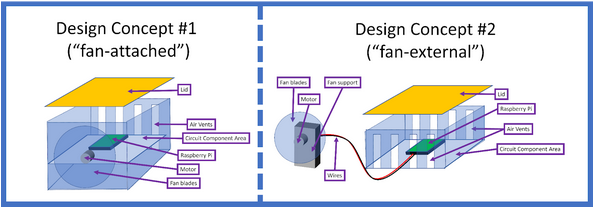
\includegraphics[width=0.4\textwidth]{designCategories}
  \caption{Design categories.}
  \label{designCategories}
\end{wrapfigure}
\subsection{Convergence}
Design concepts were separated into two categories: “fan-attached” and “fan-external” designs (Figure 1). Using the Idea Advocate convergence tool, we converged on a final “fan-attached” design due to the greater integration of system components. However, after creating a CAD model and slicing it for 3D printing, we found the design was too large to print and put us over budget by \$0.15. With this information, the team decided to use the “fan-external” design, as it would cost less in materials and be physically smaller.




\section{Implementation Process}
Design implementation was divided into three categories: structural components (creating CAD models and 3D printing the case, fan blades, and motor-housing), electrical components (wiring of electrical components, the sensor, actuator, and the MCU), and software development (writing code to interface with the raspberry pi and the sensor).

\subsection{Structural Implementation}
Some key base design features we included in our case were:
\begin{itemize}
    \item functional fan blades
    \item DC motor housing
    \item breadboard stabilization
    \item closable lid
    \item port opening for USB
    \item breadboard covering hides wiring for aesthetics, durability, and electrical safety
\end{itemize}
Drawing on lessons we learned from Widget Lab 1, we created the base to accommodate all system components first, then added design-specific elements (like the sliding lid, breadboard supports, and ventilation areas).

After implementing these features, we optimized the system to meet budgetary and infrastructure constraints. As a result, we decided use elements of our earlier “fan-external” designs by reducing the size of the fan detaching it from the case. The height and width of the case were shortened significantly to reduce material costs and make the design printable using U of T infrastructure. 

Using this iterative design process enabled us to test system manufacturability at multiple points in the design cycle. Prioritizing structural system simplicity aided us in this process, as we could quickly modify case components based on our manufacturing feedback. Some process images of the CAD models via Autodesk are provided in Figures \ref{fig:firstStructuralDesign} and \ref{fig:finalStructuralDesign}.

\begin{figure}[h]
    \centering
    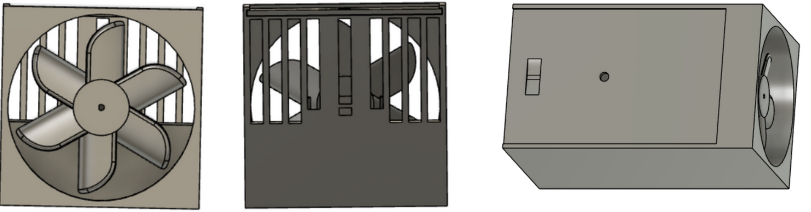
\includegraphics[width=0.5\textwidth]{firstStructuralDesign}
    \caption{Our first structural design. It was almost 2 times larger than our final design.}
    \label{fig:firstStructuralDesign}
\end{figure}
\begin{figure}[h]
    \centering
    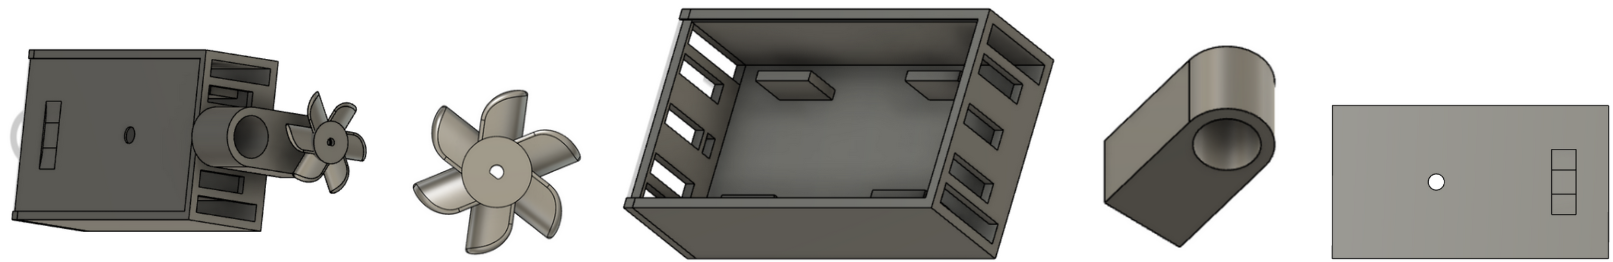
\includegraphics[width=0.8\textwidth]{finalStructuralDesign}
    \caption{Our final structural design, consisting of 4 separate components.}
    \label{fig:finalStructuralDesign}
\end{figure}



\subsection{Circuit Implementation}
\begin{figure}
    \centering
      \begin{subfigure}{0.45\textwidth}
        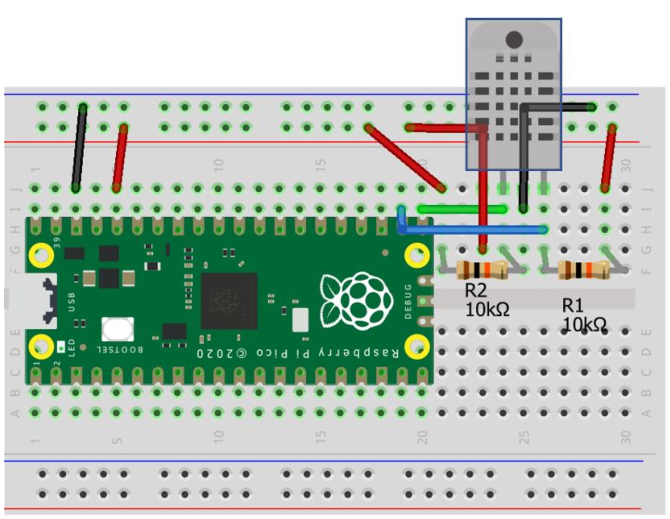
\includegraphics[width=\linewidth]{circuitDiagramSensor}
        \caption{Circuit diagram for the AM2320 temperature/humidity sensor.}
        \label{circuitDiagramSensor}
      \end{subfigure}
      \begin{subfigure}{0.40\textwidth}
        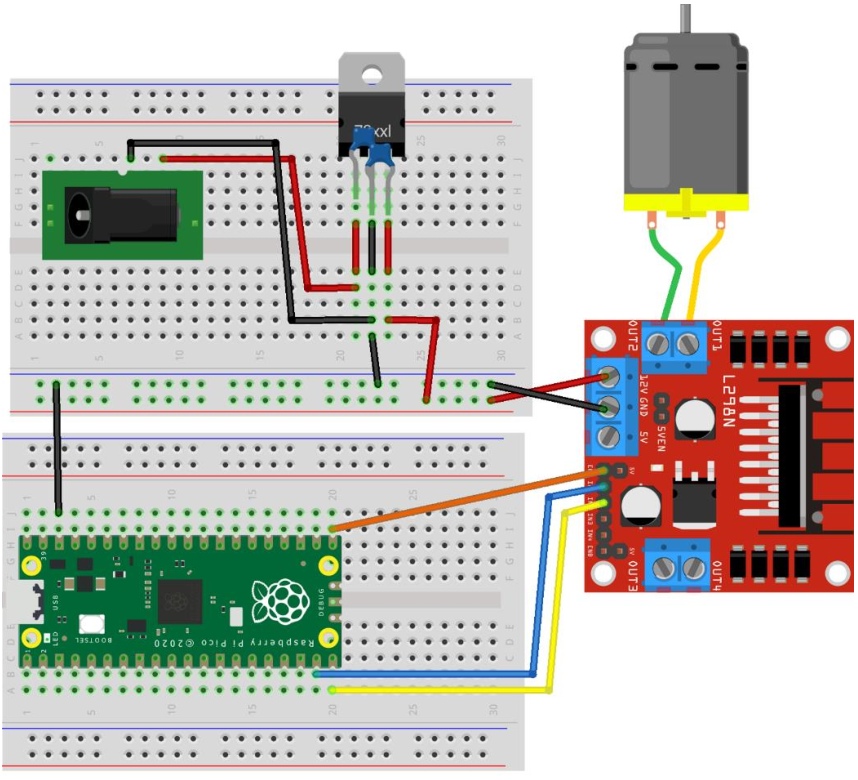
\includegraphics[width=\linewidth]{circuitDiagramMotor}
        \caption{Circuit diagram for the DC motor.}
        \label{circuitDiagramMotor}
      \end{subfigure}
    \caption{Circuit diagrams.}
    \label{circuitImplementation}
\end{figure}

The electrical portion of the prototype is composed of two parts (sensor and actuator). The sensor portion consists of a Raspberry Pi Pico, digital temperature humidity sensor (AM2320), two 10k resistor, and solid-core wires. The actuator portion consists of a DC motor along with the motor driver (L298N), barrel-to-breadboard connector, 5V regulator, 0.1 µF capacitor, 0.33 µF capacitor, 12V power supply, and solid-core wires.

\begin{wrapfigure}{r}{0.48\textwidth}
    \centering
    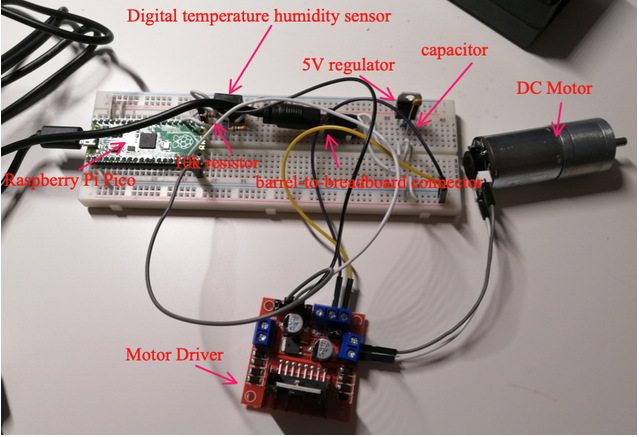
\includegraphics[width=0.45\textwidth]{finalCircuitPrototype}
  \caption{Final circuit prototype.}
  \label{finalCircuitPrototype}
\end{wrapfigure}

Through referencing Figure \ref{circuitImplementation}, we connected both the DC motor and digital temperature/humidity sensor to the same breadboard. We used a single breadboard (instead of two), to reduce the number of parts and keep more system components structurally connected. The required interior case volume was also reduced after using a single breadboard. Solid copper wires were used instead of jumper cables, as this would increase the clarity of the whole circuit due its customizable
length and further reducing space inside the case. Two jumper wires are used instead of the six-wire connector (provided for the DC motor) for connecting the DC motor to the motor driver. This reduced the number of unconnected wires and increased circuit clarity. The final circuit prototype is shown in Figure \ref{finalCircuitPrototype}.

\subsection{Code Implementation}
The provided code in Widget Lab 2 for both the DC motor and the digital temperature/humidity sensor was modified to turn the motor based on the digital temperature information.

The code for rotating the motor was copied from Section 14 of Lab 2. Since we only need the motor to turn in one direction for the fan, we removed the code that turns the motor counter clockwise. Also, since the motor runs depending on the output of the temperature/humidity sensor, we removed all code that limited the amount of time the motor ran for (i.e., less than 9 cycles). In addition to spinning when the temperature is too light, the motor needs to stop when the temperature is sufficiently low. However, we were unsure how to do this based on our DC motor experience from the prelab. Using the logic from Lab 2, we originally thought of using the ‘time.sleep()’ function. However, we soon realized that since ‘time.sleep()’ completely stops the program, it would be impossible for the code to iteratively check the temperature to run. Therefore, we arrived at the solution of simply setting the spin speed of the motor to zero to stop it. 

For the temperature/humidity sensor, we needed to read the output value of the sensor. All the code for this function was provided in Section 8 of Lab 2 and reused. 

Combining the two code bases together only required a standard ‘if-else’ statement. We checked if the temperature was above a certain value. If it was, we ran the code for rotating the motor. If it wasn’t, we ran the code that stopped rotating the motor. Thinking ahead to the testing and debugging process, we printed out the temperature read by the sensor every cycle through the loop, and placed print statements in the ‘if’ and ‘else’ cases to see if the code for each case was running. We also used the ‘time.sleep()’ function to sleep the program for 1 second every loop to give us time to read the outputs of our print statements. The implemented code can be found in Appendix \ref{code}.






\section{Evaluation Process}
Based on our testing of the air ventilation system, the change of actuator state due to temperature, and the success of the structural system in containing all components, we have concluded that the system is successful.

\begin{figure}
    \centering
      \begin{subfigure}{0.43\textwidth}
        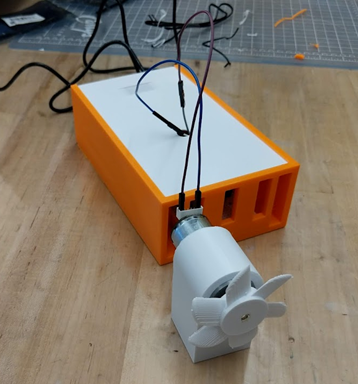
\includegraphics[width=\linewidth]{finalPrototypeOutside}
        \caption{External view.}
        \label{finalPrototypeOutside}
      \end{subfigure}
      \begin{subfigure}{0.34\textwidth}
        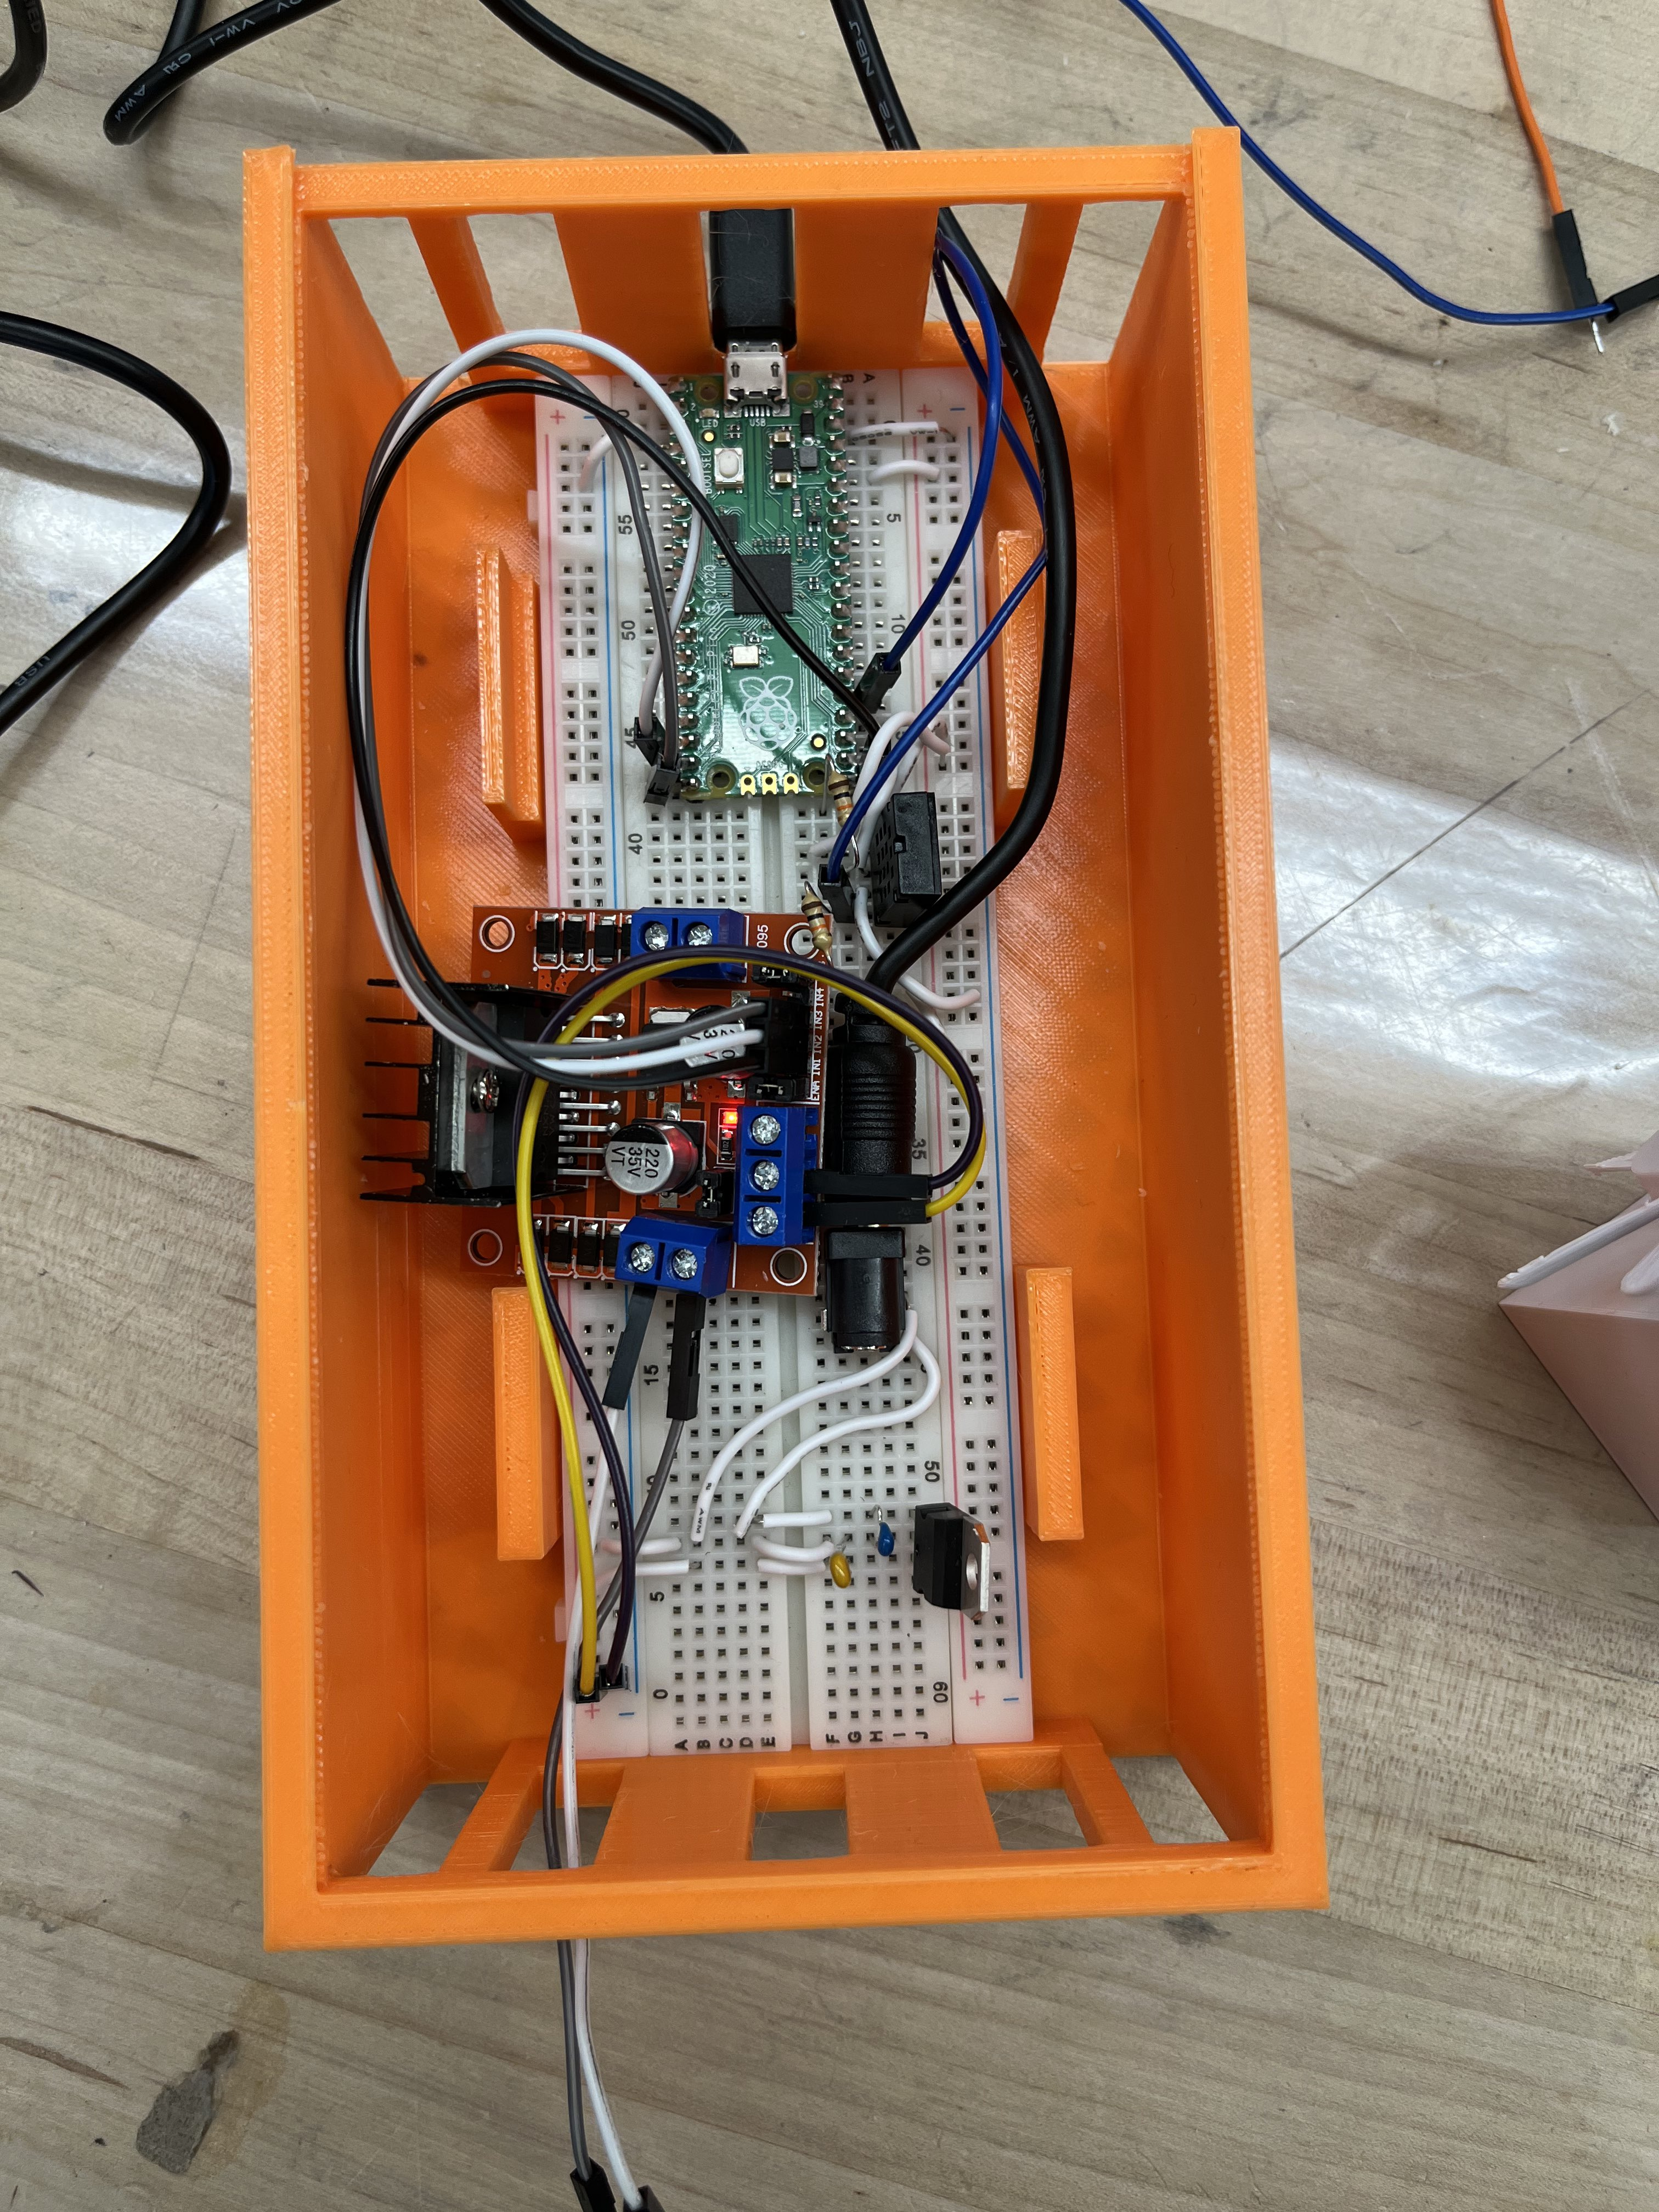
\includegraphics[width=\linewidth]{finalPrototypeInside}
        \caption{View of the internal circuitry.}
        \label{finalPrototypeInside}
      \end{subfigure}
    \caption{Our final prototype design.}
    \label{finalPrototype}
\end{figure}

Two sessions for testing and evaluation of the final prototype design, shown in Figure \ref{finalPrototype}, were conducted. 
In the first meeting, the team finalized both the electronics and code implementation, and replaced jumper wire connections with copper wires that lay flatter against the breadboard. The team was able to generate video evidence of this event. The threshold temperature was set to 25°C, where anything above this temperature would cause the motor (fan) to turn. If the sensor registered a temperature at or below 24.9°C, the motor/fan to stop. Temperature was raised by holding the sensor and decreased by manually fanning the air surrounding the sensor.

The second meeting was conducted after receiving our 3D-printed structural components including the case, the motor housing unit, and the fan. After minor structural changes were implemented to improve access to the Raspberry Pi USB port, the breadboard and circuitry were inserted. Due to the ambient room temperature in MYFab, the threshold temperature was increased to 26°C for ease of testing. Additionally, the modes of heating and cooling were refined, as holding the sensor was not the safest or fastest way to increase the temperature. We used a heat gun from MYFab to increase system temperature from a safe distance. Lowering the temperature was conducted with an electric fan. This triggered both actuator states in the assembled system (motor on/off) and proved that the air vents worked to effectively convey external temperature information to the temperature sensor. 

Though all videos taken during meeting and evaluation showcase the functionality of the product, they also display distinct steps towards optimizations of testing. Increasing the variability and ease of control over surrounding temperatures enabled us to conduct quicker and more efficient verifications of the system’s feasibility. 

\href{https://youtu.be/O1di9BagJPE}{Video 1, First Meeting}: prototype and successful testing without structural components. Threshold temperature was set at 25°C. Temperature raised with physical contact, temperature lowered with manual fanning.

\href{https://youtu.be/K5c0lNJ9v3A}{Video 2, Start of second meeting}: prototype and successful testing with structural components. Threshold temperature was set at 26°C. Temperature raised with hand around case, temperature lowered with electric fan.

\href{https://youtu.be/0W4DSpp6AJQ}{Video 3, End of second meeting}: prototype and successful testing with structural components. Threshold temperature was set at 26°C. Temperature raised with heat gun, temperature lowered with electric fan.


%\begin{figure}
    %\centering
      %\begin{subfigure}{0.45\textwidth}
        %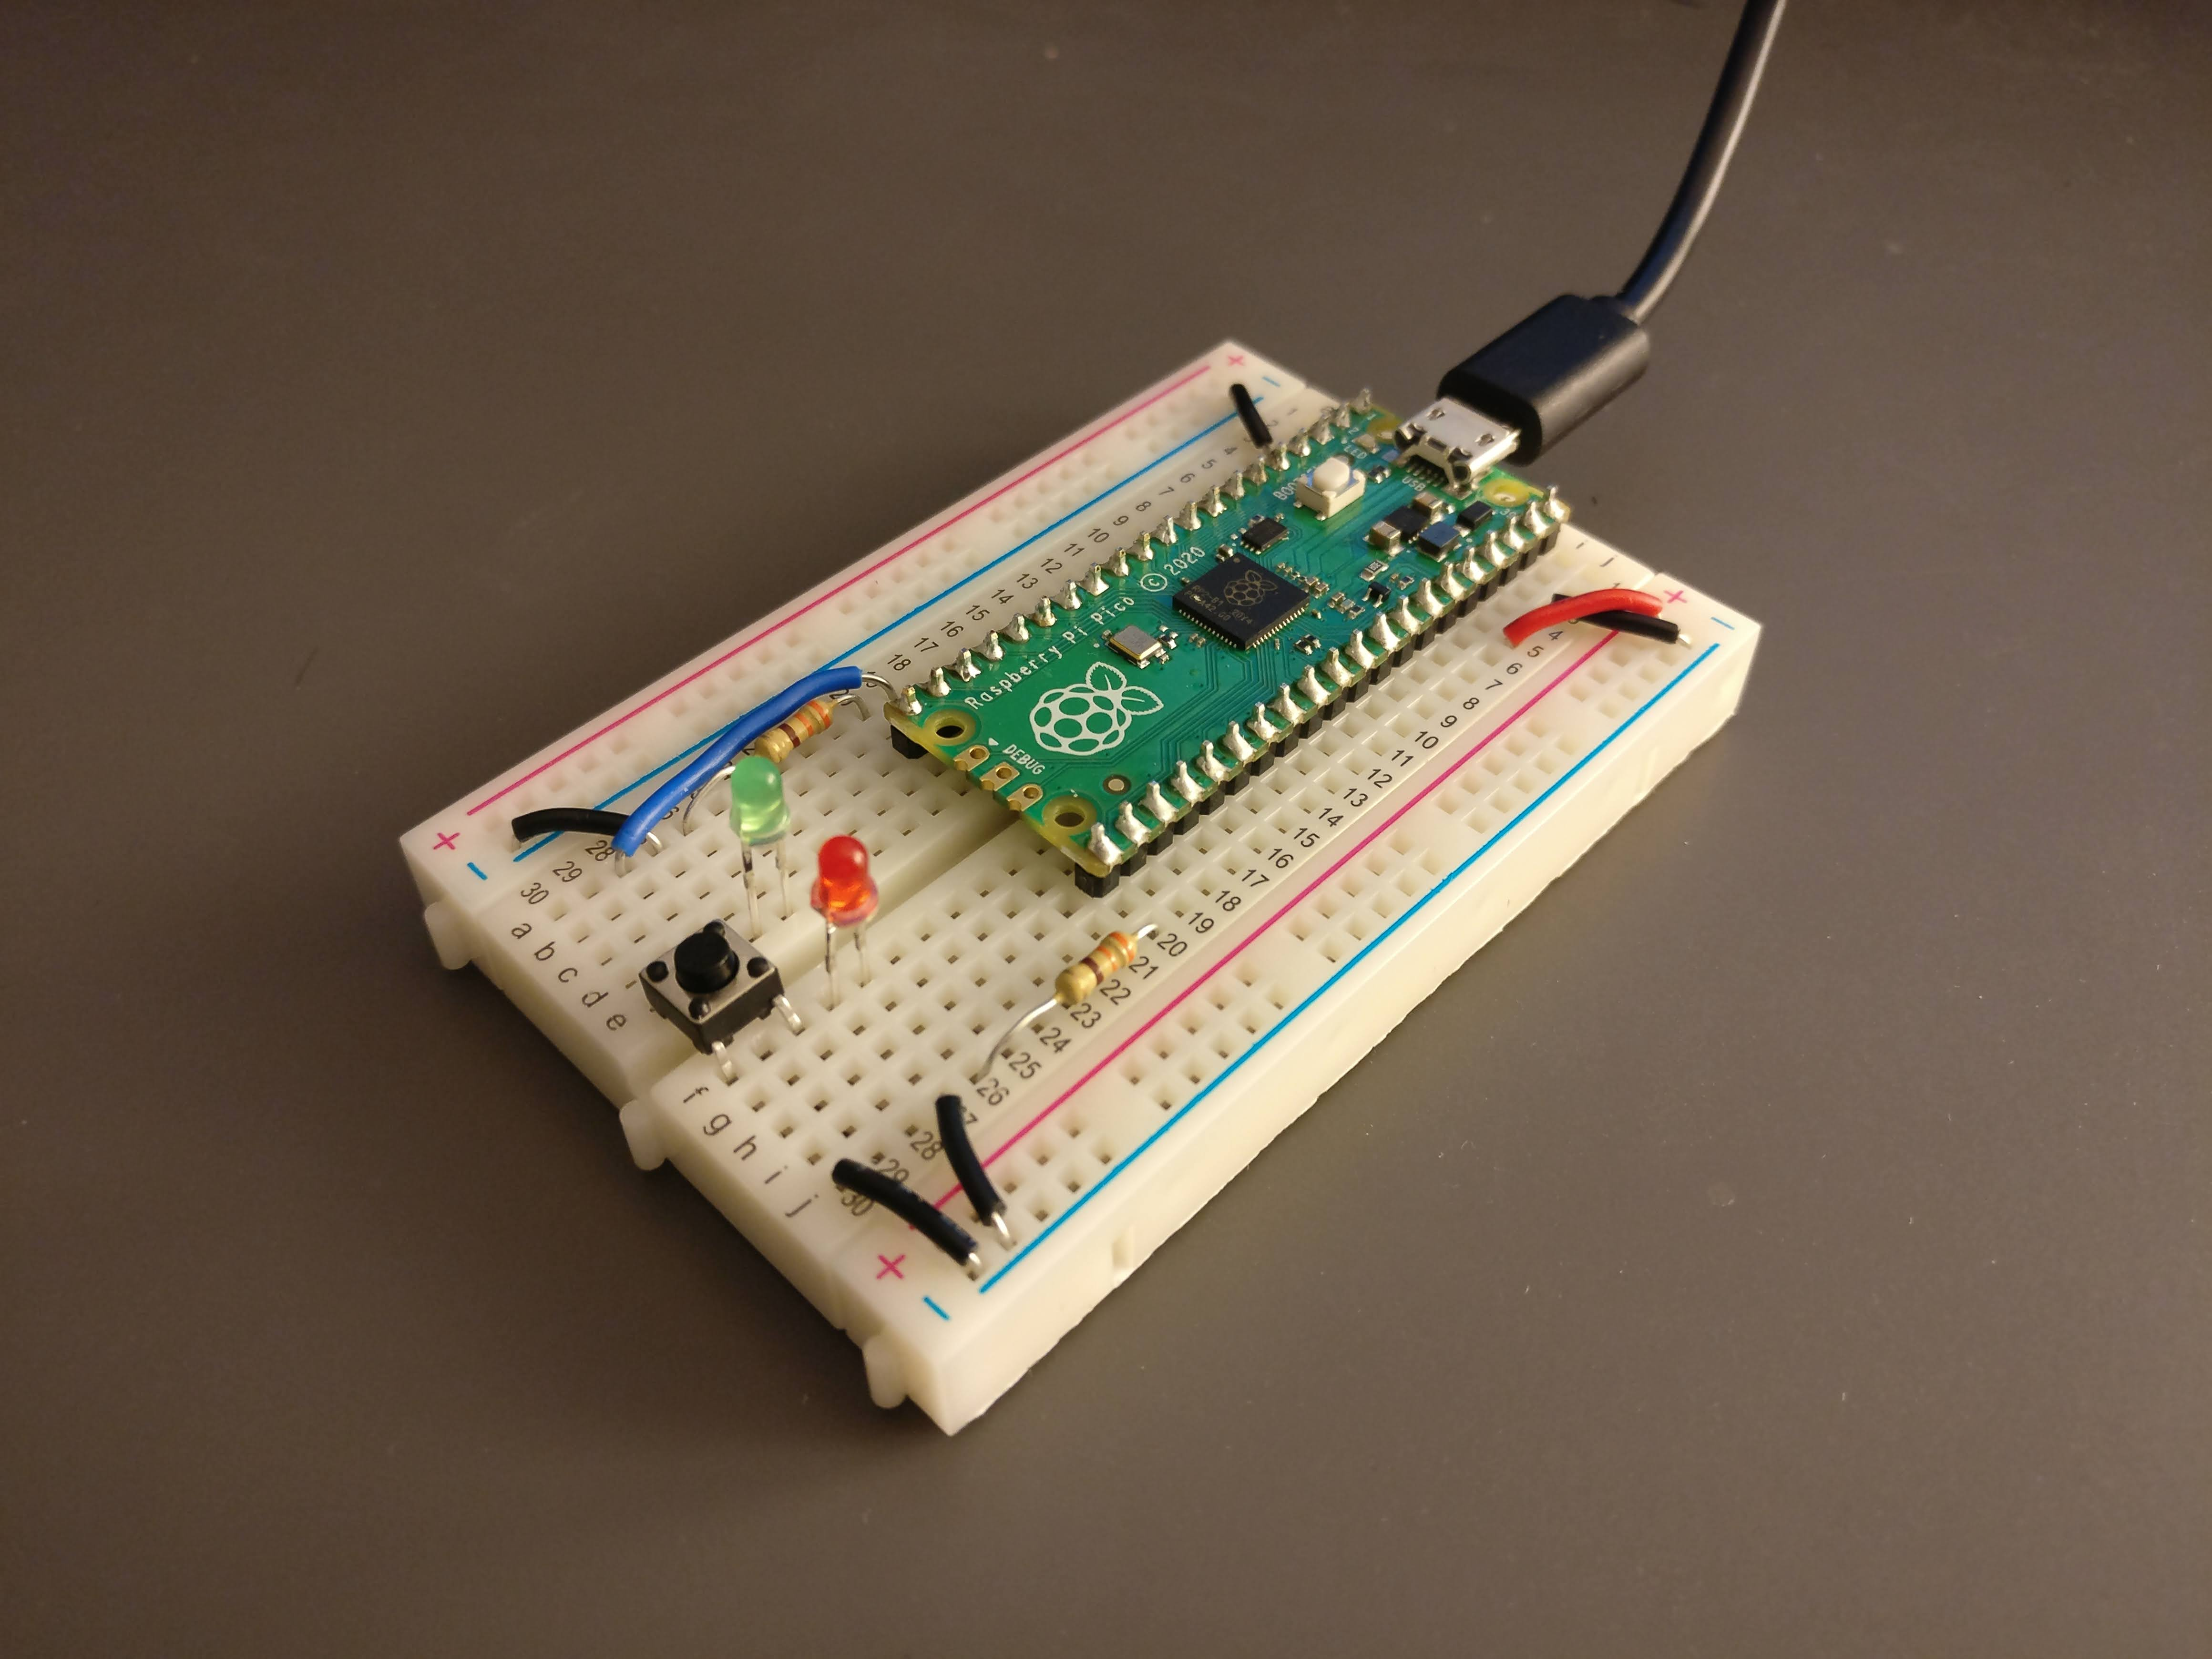
\includegraphics[width=\linewidth]{figures/finaldiagview.jpg}
        %\caption{Angled view}
        %\label{finaldiagview}
      %\end{subfigure}
      %\begin{subfigure}{0.25\textwidth}
        %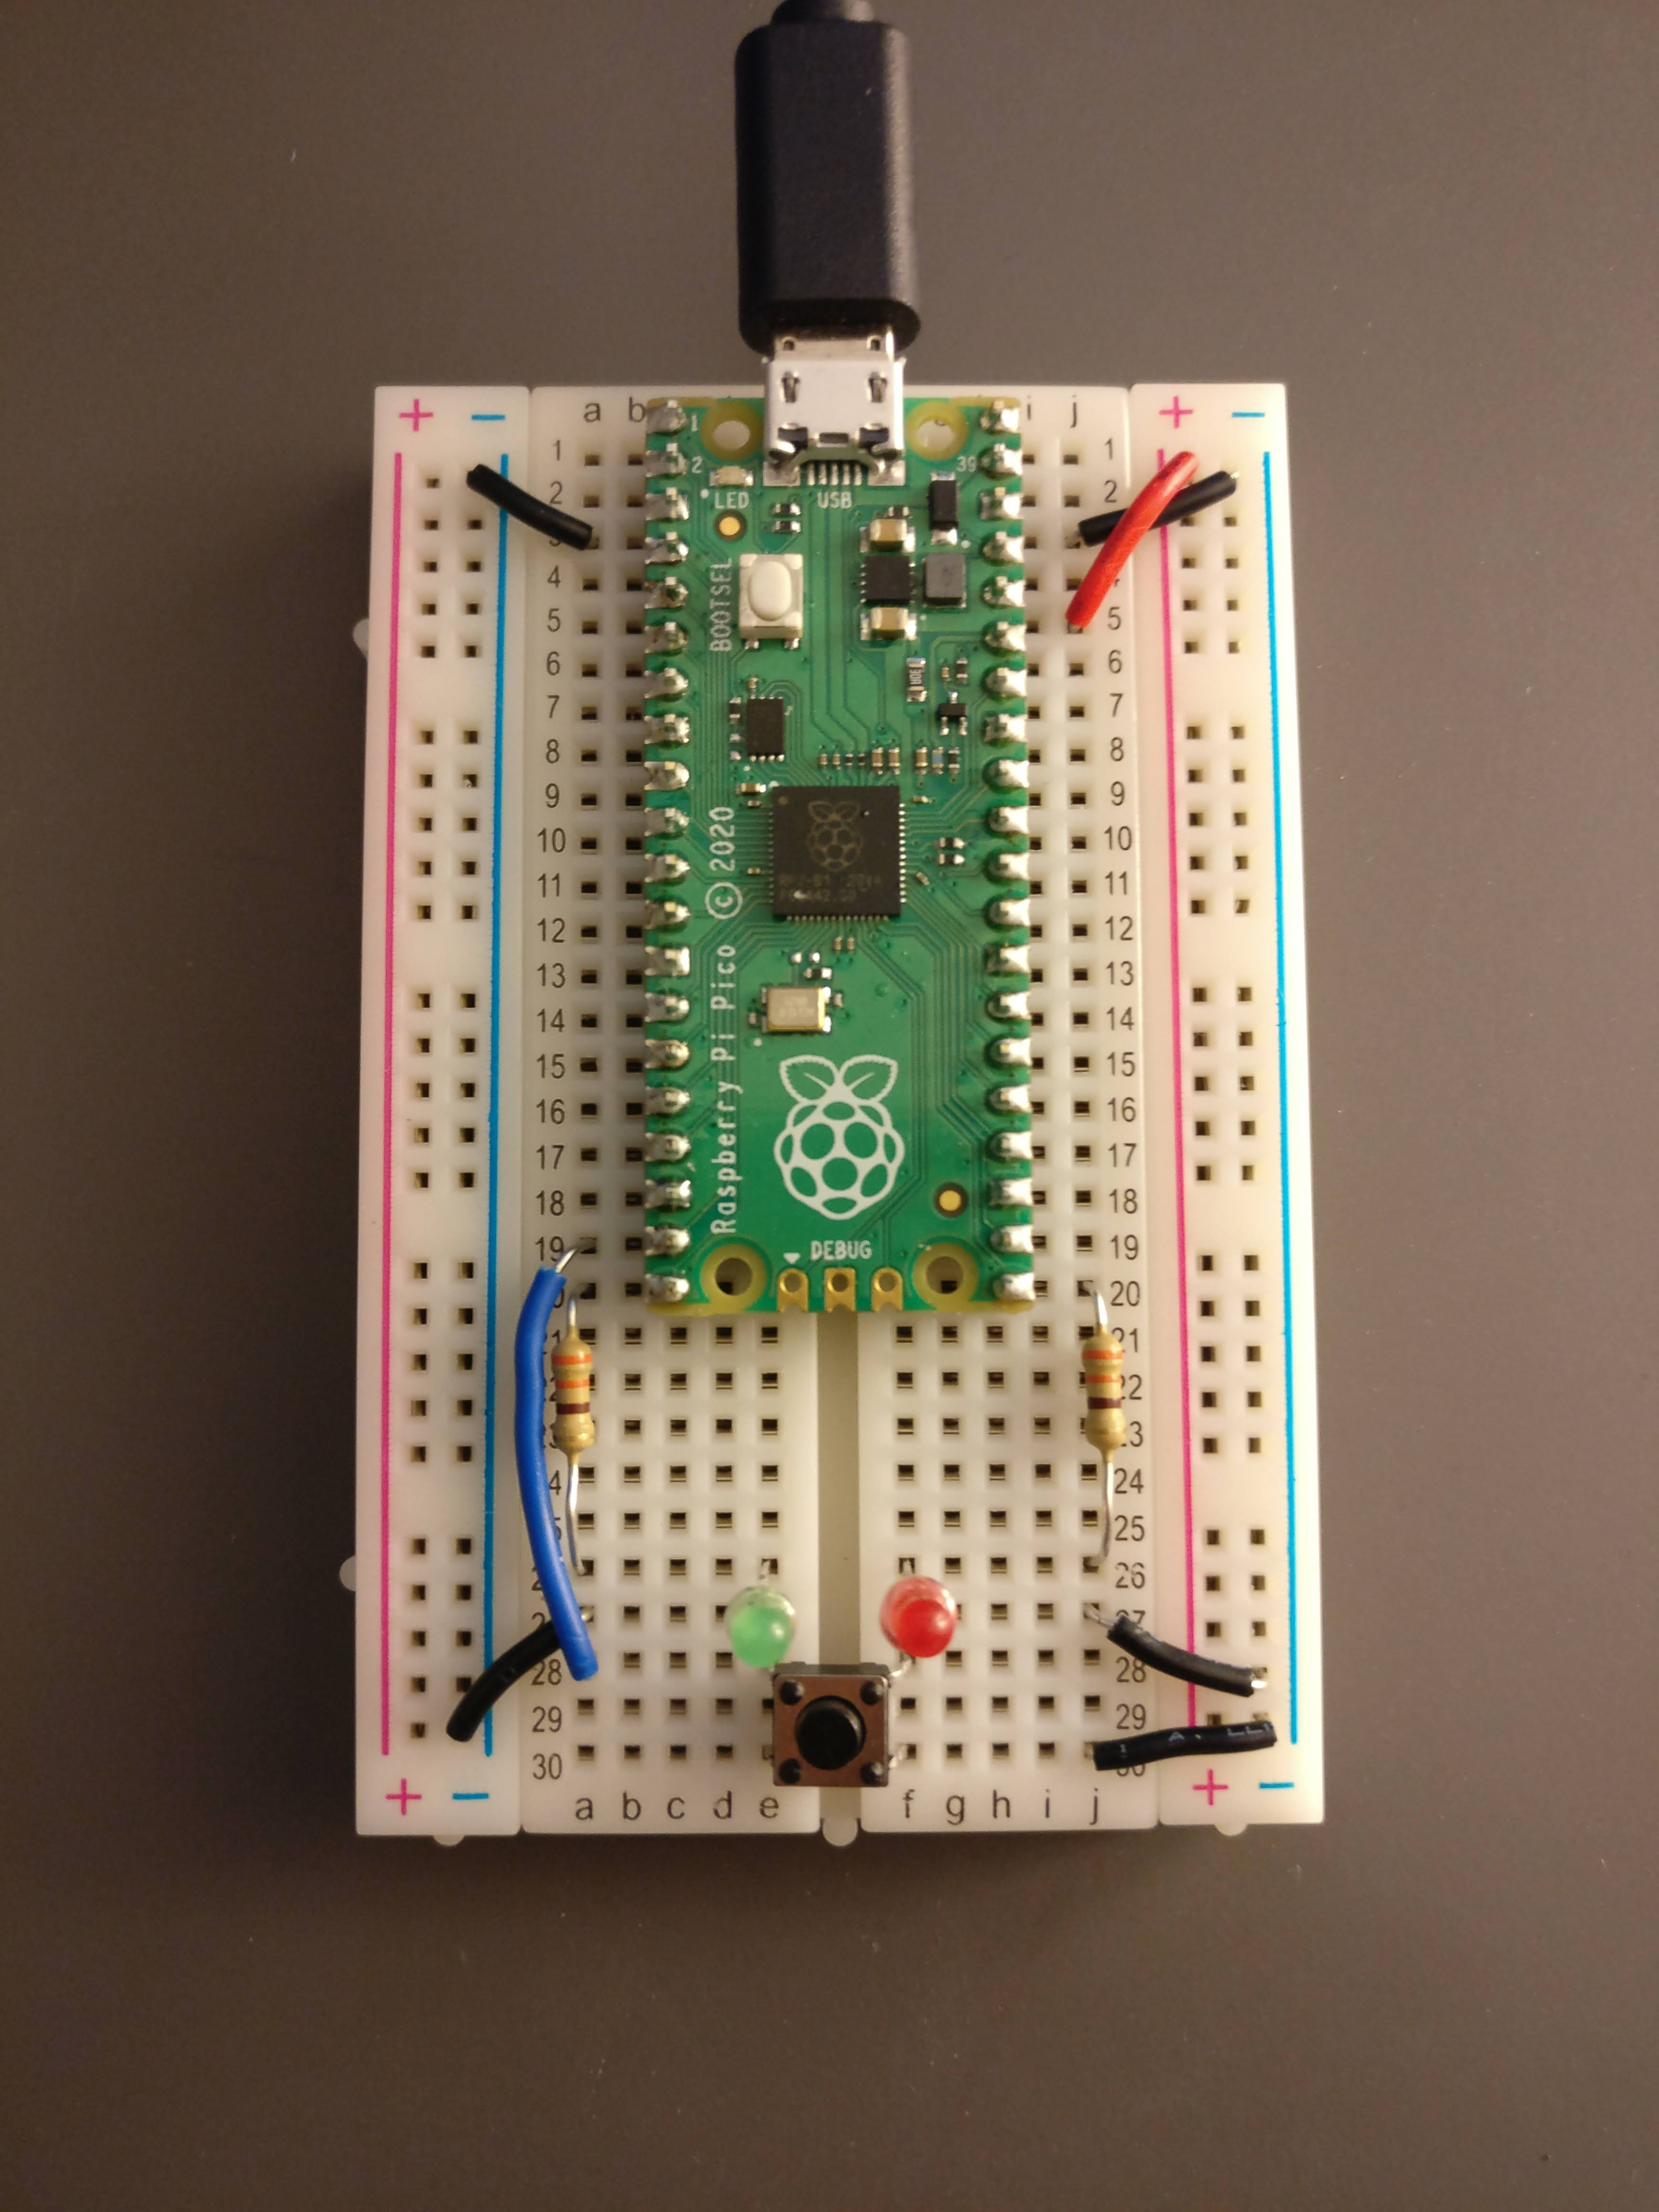
\includegraphics[width=\linewidth]{figures/finaltopview.jpg}
        %\caption{Top view}
        %\label{finaltopview}
      %\end{subfigure}
    %\caption{Final system prototype}
    %\label{finalprototype}
%\end{figure}




\section{Individual contributions}
Throughout this assignment, I mainly focused on the design, implementation, and debugging of the software. 
In the process of designing the code for the system, I was able to quickly identify that the code would be a simple combination of the programs we used in Widget Lab 2 for the motor and the temperature/humidity sensor. 
I was then responsible for implementing the code, which was a very straightforward process using an 'if-else' statement.  
I also thought of the idea of setting the motor speed to zero to stop it instead of using the 'time.sleep()' function.
During the testing/evaluation process, the software was run on my laptop, and so I was responsible for most of the debugging.
Beyond the software aspect, I contributed to the electrical and structural aspects too. 
I helped the team implement some of the initial wiring on the breadboard. I also used the datasheets provided to identify which pins to use on the DC motor since there were 6 in total, when we only needed to use 2.
In the design process of the structural aspect, we held numerous meetings where I contributed some of my ideas and gave feedback on preliminary design concepts.



\section{Reflection on learning process}

\subsection{What I learned}
The main things I learned from this lab came from my involvement in the electrical portions of the lab. Since I am already familiar with Python and other software languages, there was very little I was unfamiliar with when working on the code. But when helping the team out on the electrical portions of the lab, I learned a lot since my exposure to hardware in the past has been fairly limited. Setting up all the different devices (temperature/humidity sensor, DC motor,
thermistor, etc.) was a very new and foreign process to me, and implementing them required a lot of reading of the provided datasheets. Consequently, I learned a lot about how these devices work and how to wire them correctly in order to communicate with the Raspberry Pi Pico.

\subsection{What helped my learning}
The datasheets provided in the lab instructions greatly assisted my learning process. When I did not understand how something worked, I immediately looked to the datasheets, which have proved to be very useful as I have learned a lot. Sometimes, when the datasheets were not sufficient, I would consult the Internet which has always been one of my main sources of information. My team members also helped a great deal. We all have different areas that we are more specialized in, so whenever I
encountered struggles in understanding content, I would often ask for help from my team since usually one of them is likely to be knowledgable regarding that content.


\subsection{Future interests and previous experiences}
Again, similarly to Lab 1, areas related to this lab that I’m interested in learning more about primarily include the hardware aspects of the lab, as well as how to communicate with them through software. Learning about the different sensors and actuators, wiring them, and using software to control them was the most enjoyable part of the lab for me.

My experience with this lab mainly reminds me of the programming courses I've taken in the past. Since the language used was Python, I was able to use Python learned from high school courses and ESC180 when working on the software aspect of the widget. Although I was not involved, the structural aspect of the lab also reminded me of a design and technology course I took in high school, where we learned to model small physical structures in AutoCAD. Beyond the software and CAD modelling, I was fairly unfamiliar with the content of the lab as I've had little academic and professional experience working with sensors and actuators. 

\subsection{What I would do differently}
In the future, I would try to get more involved in the hardware aspects of the lab since there is a lot of room for learning and development in that field for me. Since I primarily focused on the software in this assignment, I feel as though I did not fully maximize my learning experience. Otherwise, this lab went smoothly for me and I had a great time working with my team as well. I look forward to collaborating with them again and learning more.






\newpage


% \begin{thebibliography}{99}

% \bibitem{Bostrom}
% Bostrom, Nick. 2014. \textit{Superintelligence: Paths, Dangers, Strategies.} New York: Oxford University Press.

% \end{thebibliography}



\section{Appendix}

\subsection{System Code} \label{code}
\begin{lstlisting}[language=Python, caption=Python code for the widget]
'''
ESC204 2022W Widget Lab 2 Assignment
'''

import board
import bitbangio
import adafruit_am2320
import time
import digitalio
import pwmio
import sys

# set up I2C protocol
i2c = bitbangio.I2C(board.GP19, board.GP18)
dhtDevice = adafruit_am2320.AM2320(i2c)

# set up logic inputs to motor driver ("step" and "pulse") as outputs
in1 = digitalio.DigitalInOut(board.GP14)
in2 = digitalio.DigitalInOut(board.GP15)
in1.direction = digitalio.Direction.OUTPUT
in2.direction = digitalio.Direction.OUTPUT

# set up PWM output to motor driver
ena = pwmio.PWMOut(board.GP16)

# set initial duty cycle, direction, and step commands
ena.duty_cycle = 0
in1.value = False
in2.value = True

while True:

    try:
        print("hello")
        # Print the values to the serial port
        temperature_c = dhtDevice.temperature
        time.sleep(0.5)
        humidity = dhtDevice.relative_humidity
        print("AM2320 Temp: {:.1f} C Humidity: {}%".format(temperature_c,humidity))

    except RuntimeError as error:
        # Errors happen fairly often, DHT's are hard to read, just keep trying to run/power cycle Pico
        print(error.args[0])


    if temperature_c >= 25:
        # rotate motor clockwise
        in1.value, in2.value = (False, True)
        ena.duty_cycle = 65535
        print("Motor is rotating CW")

    else:
        ena.duty_cycle = 0 # set speed to zero
        print("Motor isn't rotating")

    time.sleep(0.5)
\end{lstlisting}









\end{document}
